% !TeX root = ../main.tex
% Chapter 1 -- General introduction.  This sample shows the main formatting features:
% numbered headings, citations, a figure, a table, an equation, a block quote and a footnote.
% Replace everything below the \label line with your own text.
\chapter{GENERAL INTRODUCTION}
\label{ch:intro}

\section{Using This Template}

Each chapter lives in its own file in the \texttt{chapters/} folder and is included from \texttt{main.tex}. The chapter heading (``CHAPTER 1'' followed by the title) is centered in capitals at the top of a new page, as the Graduate School requires. Text is double-spaced with a \textonehalf-inch paragraph indent, and every page carries a centered page number inside the 1-inch bottom margin.

Cite references with \verb|\cite{key}|; numbered superscript citations are produced in the order in which sources are first cited\cite{Ma2010three,Balzarotti2017nanometer}. Several sources cited together are sorted and compressed into a range\cite{Betzig2006imaging,Ma2010three,Balzarotti2017nanometer,Lin2019structure}. The reference list at the end of the dissertation is generated by BibTeX from \texttt{references.bib}.

\subsection{Figures}

Figures are numbered by chapter (Figure~\ref{fig:intro:example}). Give every figure a short title in square brackets: that title appears in the List of Figures, while the full legend appears under the figure. Captions are single-spaced and must not use type smaller than 10 points.

\begin{figure}[tbp]
\centering
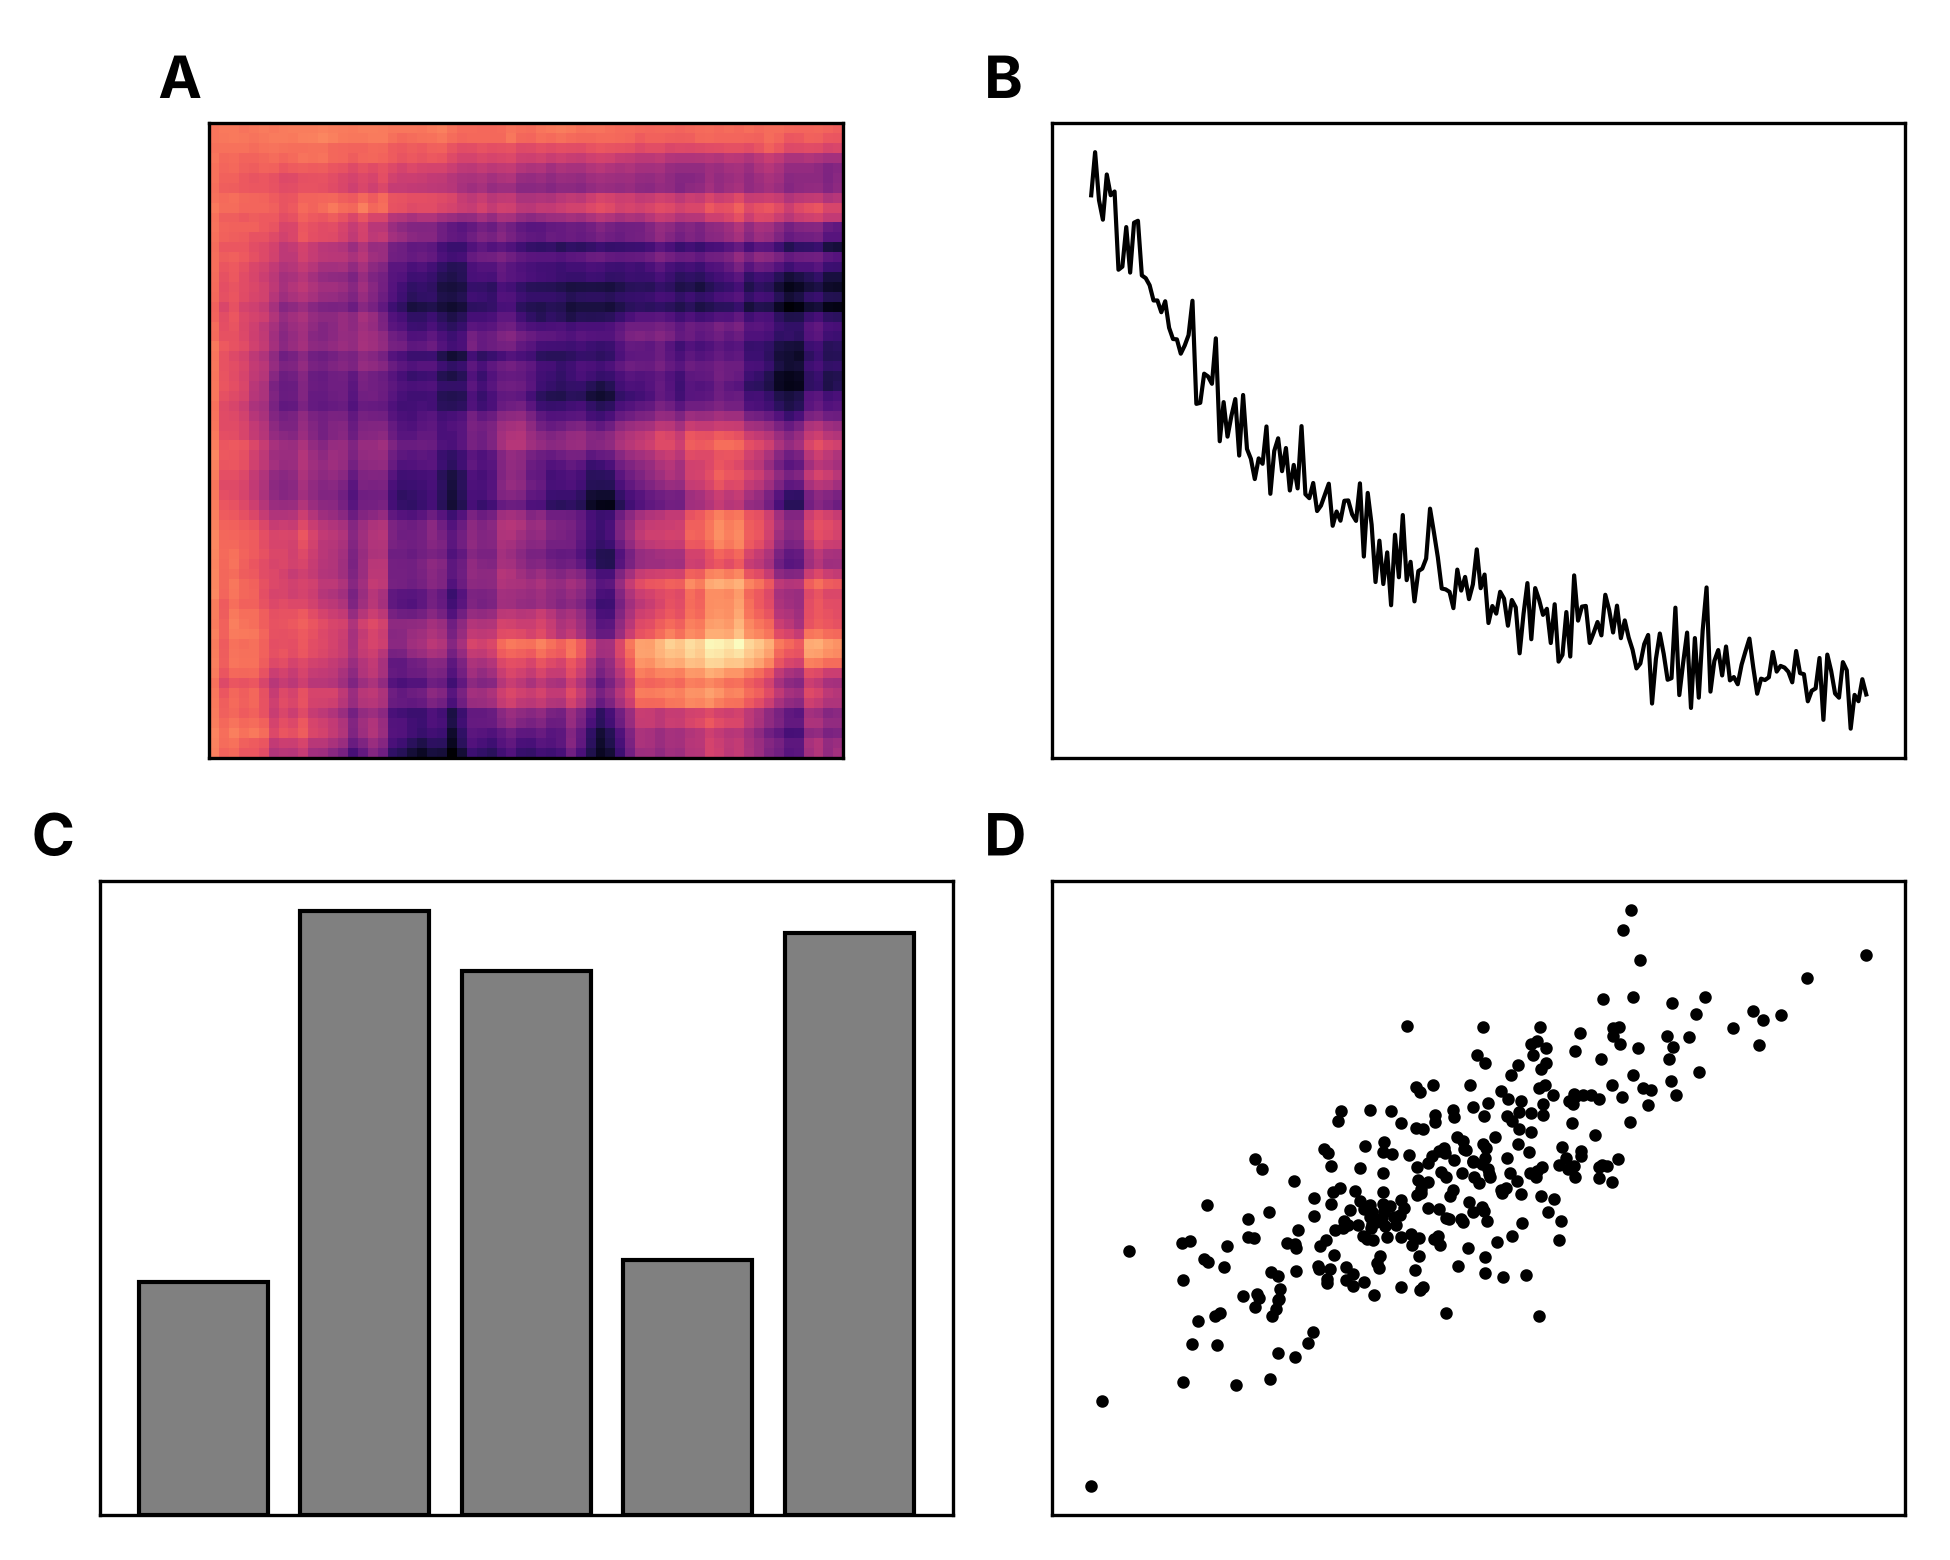
\includegraphics[width=\textwidth,keepaspectratio]{figures/example-figure.png}
\caption[Example of a multi-panel figure]{\textbf{Example of a multi-panel figure.} \textbf{(A)} Panel A description. \textbf{(B)} Panel B description. \textbf{(C)} Panel C description; bars show the mean \textpm{} s.d. of $n = 3$ independent experiments. \textbf{(D)} Panel D description. Scale bar, 1~\textmu m.}
\label{fig:intro:example}
\end{figure}

\subsection{Tables}

Tables are also numbered by chapter (Table~\ref{tab:intro:example}). The \verb|\tablesmall| command reduces the type size of a wide table by one step while keeping it at or above the 10-point minimum.

\begin{table}[tbp]
\centering
\caption[Example of a data table]{\textbf{Example of a data table.} Values are mean \textpm{} s.d.}
\label{tab:intro:example}
\begin{tabular}{@{}lccc@{}}
\toprule
\textbf{Condition} & \textbf{Diffusion coefficient (\textmu m\textsuperscript{2}/s)} & \textbf{Dwell time (ms)} & \textbf{$n$} \\
\midrule
Control   & 0.85 \textpm{} 0.10 & 4.2 \textpm{} 0.6 & 512 \\
Treatment & 0.42 \textpm{} 0.08 & 7.9 \textpm{} 1.1 & 488 \\
\bottomrule
\end{tabular}
\end{table}

\subsection{Equations}

Equations are numbered by chapter, as in Equation~\eqref{eq:intro:msd}:
\begin{equation}
\text{MSD}(t) = \left\langle \left[ r(t_0 + t) - r(t_0) \right]^2 \right\rangle = 2dDt,
\label{eq:intro:msd}
\end{equation}
where $d$ is the number of dimensions and $D$ is the diffusion coefficient.

\section{Other Text Elements}

\subsection{Block Quotations}

Quotations of 40 or more words are set as a block, single-spaced, indented \textonehalf{} inch from both margins, and without quotation marks. The source citation follows the closing punctuation:

\begin{quote}
This is an example of a long quotation of forty words or more. It is set as a free-standing block of text, single-spaced and indented one-half inch from both the left and the right margins, with no surrounding quotation marks, exactly as the Dissertation and Thesis Handbook requires.\cite{Lin2019structure}
\end{quote}

Shorter quotations are integrated into the text and enclosed in quotation marks.

\subsection{Notes}

Most biology dissertations do not need footnotes, but the template formats them as the Handbook requires.\footnote{Footnotes are set in the same type size as the text, single-spaced within a note, with a blank line between notes and the first line indented one-half inch.}

\subsubsection{A third-level heading}

Use at most three heading levels. Only chapters, sections and subsections appear in the Table of Contents; to include third-level headings, change \verb|\setcounter{tocdepth}{2}| to 3 in \texttt{templethesis.sty}.
